\tikzsetnextfilename{figures/logs/logs}
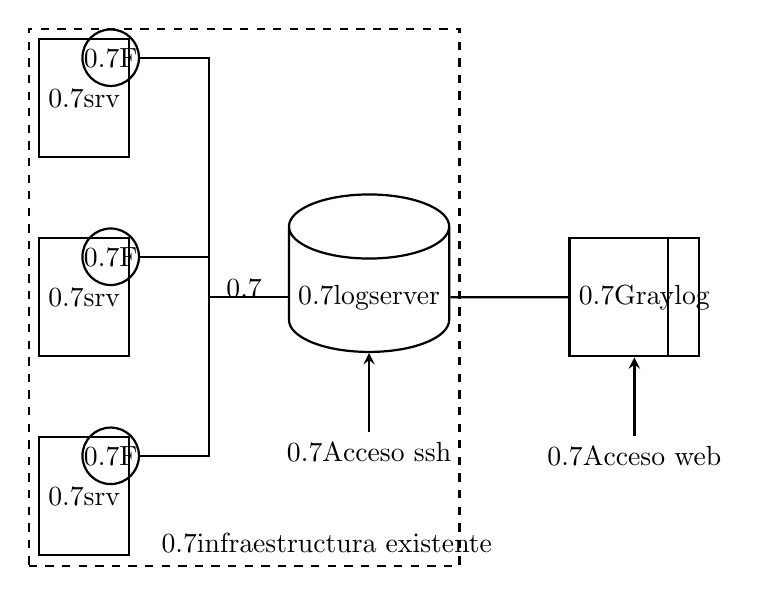
\begin{tikzpicture}[
    font=\relscale{0.7},
    thick
  ]
\usetikzlibrary{positioning,fit,calc,shapes}
\def\nw{1cm}

\tikzstyle{bignode}=[minimum height=1.5*\nw,minimum width=\nw]

\node[draw,bignode] (srv1) {srv};
\node[draw,bignode,below= of srv1] (srv2) {srv};
\node[draw,bignode,below= of srv2] (srv3) {srv};

\node[circle,draw,minimum height=.3*\nw,minimum width=.3*\nw,inner sep=0mm] at ($ (srv1.north east) - (.25*\nw,.25*\nw) $) (f1) {F};
\node[circle,draw,minimum height=.3*\nw,minimum width=.3*\nw,inner sep=0mm] at ($ (srv2.north east) - (.25*\nw,.25*\nw) $) (f2) {F};
\node[circle,draw,minimum height=.3*\nw,minimum width=.3*\nw,inner sep=0mm] at ($ (srv3.north east) - (.25*\nw,.25*\nw) $) (f3) {F};

\node[draw,cylinder,bignode,minimum height=2*\nw, node distance=2*\nw,shape border rotate=90, shape aspect=0.4, right = of srv2] (logserver) {logserver};

\node[draw,bignode,rectangle split,rectangle split horizontal,rectangle split parts=2, node distance=1.5*\nw,text width=\nw,align=center,right = of logserver] (graylog) {Graylog};

\coordinate (aux) at ($ (logserver.west) - (\nw,0) $);

\node[fit=(srv1.north west)(srv3.south west)(logserver.east),draw,dashed] (ex) {};
\node[] at ($ (ex.south east) + (-1.7*\nw,.3*\nw) $) {\e{infraestructura existente}};

\draw[-] (f1) -| (aux) -- (logserver.west);
\draw[-] (f2) -| (aux) -- (logserver.west);
\draw[-] (f3) -| (aux) -- (logserver.west);

\draw[-,draw] (logserver) -- (graylog.west);

\node[below=of logserver] (ssh) {Acceso ssh};
\node[below=of graylog] (web) {Acceso web};

\draw[-stealth] (ssh) -- (logserver.south);
\draw[-stealth] (web) -- (graylog.south);

\end{tikzpicture}
